% !TEX program = xelatex
\documentclass[10pt,letterpaper,twocolumn]{article}
\usepackage[margin=0.75in]{geometry}
\usepackage{fontspec}
\setmainfont{Latin Modern Roman}[Extension=.otf,UprightFont=lmroman10-regular,BoldFont=lmroman10-bold,ItalicFont=lmroman10-italic,BoldItalicFont=lmroman10-bolditalic]
\setsansfont{Latin Modern Sans}[Extension=.otf,UprightFont=lmsans10-regular,BoldFont=lmsans10-bold,ItalicFont=lmsans10-oblique]
\setmonofont{Latin Modern Mono}[Extension=.otf,UprightFont=lmmono10-regular,Scale=0.85]
\newfontfamily\acbold{ywft-processing-bold}[Path=../../system/public/type/webfonts/,Extension=.ttf]
\usepackage{xcolor,titlesec,booktabs,tabularx,enumitem,fancyhdr,microtype,tikz,balance}
\usepackage[numbers,sort&compress]{natbib}
\usepackage{hyperref,xurl}
\usepackage{../ac-source-bundle}
\usetikzlibrary{positioning,arrows.meta}
\definecolor{acpink}{RGB}{180,72,135}
\definecolor{acpurple}{RGB}{120,80,180}
\definecolor{acdark}{RGB}{64,56,74}
\definecolor{acgray}{RGB}{119,119,119}
\definecolor{acgreen}{RGB}{35,105,85}
\newcommand{\acdot}{{\color{acpink}.}}
\newcommand{\ac}{Aesthetic{\acdot}Computer}
\newcommand{\code}[1]{\texttt{\nolinkurl{#1}}}
\hypersetup{colorlinks=true,linkcolor=acpurple,urlcolor=acpurple,citecolor=acpurple,pdftitle={Oskie Files in Unreal Engine},pdfauthor={@jeffrey}}
\titleformat{\section}{\normalfont\bfseries\normalsize\uppercase}{\thesection.}{0.5em}{}
\titlespacing{\section}{0pt}{1em}{0.3em}
\titleformat{\subsection}{\normalfont\bfseries\small}{\thesubsection}{0.5em}{}
\titlespacing{\subsection}{0pt}{0.7em}{0.2em}
\pagestyle{fancy}\fancyhf{}\renewcommand{\headrulewidth}{0pt}
\fancyfoot[C]{\footnotesize\thepage}
\setlength{\columnsep}{1.8em}\setlength{\parskip}{0.25em}
\setlist[enumerate]{nosep,leftmargin=1.4em}
\newcolumntype{L}{>{\raggedright\arraybackslash}X}
\renewcommand{\dbltopfraction}{0.9}\renewcommand{\topfraction}{0.9}
\renewcommand{\textfraction}{0.08}
\setcounter{dbltopnumber}{2}
\emergencystretch=1.4em
\begin{document}
\twocolumn[{
\begin{center}
{\acbold\fontsize{24}{28}\selectfont\color{acdark} Oskie Files in Unreal Engine}\par
\vspace{0.7em}
\href{https://prompt.ac/@jeffrey}{@jeffrey}\par
{\small \ac{} · November 6, 2026}\par
{\small ORCID: \href{https://orcid.org/0009-0007-4460-4913}{0009-0007-4460-4913}}
\end{center}
\begin{quote}\small\noindent\textbf{Abstract.}
A \code{.oskie} file packages a game's JavaScript modules, assets, and manifest. Keeping that file as the authored object would let games made for Oskiewar travel into Unreal Engine without becoming separate Blueprint projects. This design describes an Unreal runtime plugin that embeds QuickJS, loads the Oskiewar engine, and implements its host interface. It separates a compatibility renderer, which preserves the existing projected drawing commands, from a later world-space bridge for Unreal geometry and materials. A six-stage implementation map covers bundle loading, execution, rendering, input and sound, packaged builds, and optional native scene integration. Source inspection establishes the starting architecture; no Unreal plugin or Unreal performance result is claimed. Browser dependencies, engine versioning, resource limits, and measurable acceptance gates define what it would take for the same file to keep being the same game.
\end{quote}\vspace{0.5em}
}]

\section{Keep the file}\label{sec:problem}
A \code{.oskie} file is the thing a person makes, sends, opens, and revises. Unreal should be another place to play it. Rebuilding each game as a collection of Unreal assets would move authorship away from that small object and create two games to maintain.

The initial target is narrower: import an existing-format bundle, execute its portable game code through the original Oskiewar runtime, and play it in an Unreal desktop executable. The Unreal editor can help inspect and package the game. It must not be required when someone runs it.

Oskiewar already has the useful architectural seam. Its native Xbox host embeds QuickJS and binds drawing, input, sound, and other services into JavaScript. Its browser and native hosts supply different implementations below the game. The August system report documents the earlier native fighting game and spectator architecture \citep{oskiewar}. The current renderer split describes a mix of projected primitives and retained objects across hosts \citep{split}. These are precedents for another host, not evidence that Unreal integration is complete.

The current browser player also makes the limit visible. Games can reach browser globals as well as the Oskiewar API. A file that asks \code{document} for pointer lock has an environmental dependency that a JavaScript interpreter alone does not satisfy. Section~\ref{sec:contract} defines the boundary; Sections~\ref{sec:host}--\ref{sec:map} turn it into an implementation; Section~\ref{sec:evaluation} defines the proof.

\begin{figure*}[t]
\centering
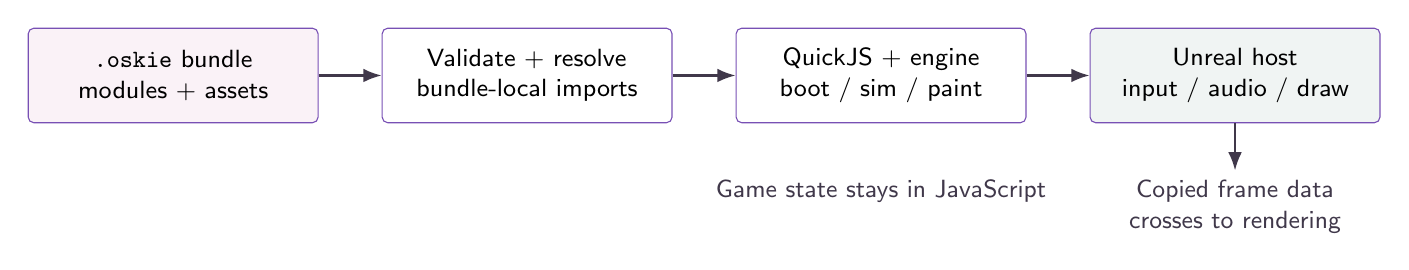
\begin{tikzpicture}[node distance=8mm,>=Latex,
 box/.style={draw=acpurple,rounded corners=2pt,align=center,font=\sffamily\small,minimum height=12mm,text width=34mm,inner sep=4pt},
 flow/.style={->,thick,draw=acdark}]
\node[box,fill=acpink!7] (file) {\texttt{.oskie} bundle\\modules + assets};
\node[box,right=of file] (load) {Validate + resolve\\bundle-local imports};
\node[box,right=of load] (vm) {QuickJS + engine\\boot / sim / paint};
\node[box,right=of vm,fill=acgreen!7] (host) {Unreal host\\input / audio / draw};
\draw[flow] (file)--(load);\draw[flow] (load)--(vm);\draw[flow] (vm)--(host);
\node[align=center,font=\sffamily\small,text=acdark,below=6mm of vm] (state) {Game state stays in JavaScript};
\node[align=center,font=\sffamily\small,text=acdark,below=6mm of host] (frame) {Copied frame data\\crosses to rendering};
\draw[flow] (host)--(frame);
\end{tikzpicture}
\caption{Proposed runtime boundary. The bundle and game logic remain portable; Unreal owns the host services. Rendering receives copied frame data, not live JavaScript objects. The editor importer is optional tooling around this path, so a packaged build can execute the same validated asset.}
\label{fig:boundary}
\end{figure*}

\section{The compatibility contract}\label{sec:contract}
\subsection{Three versions, three jobs}
The public validator recognizes JSON with \code{format: "ac.oskiewar.game"}, schema \code{version: 1}, a \code{manifest}, and a \code{files} map. Each file contains a MIME type and either text or base64 data. The entry module defaults to \code{game.mjs}. The validator limits the file count to 128 and encoded file contents to 2 MiB \citep{bundle}. A native loader should also limit the complete JSON input and decoded allocations; the existing content limit is not a complete memory budget.

Keep the schema version, runtime identifier, and engine build separate. Schema 1 describes the container. \code{oskiewar-1} identifies the game API family. The optional \code{engine} integer records an engine build; it does not by itself prove compatibility or identify exact bytes. A release lock should add the engine hash and host capability level outside the game payload, then reject an unsupported combination with a useful error.

The first Unreal milestone accepts \code{mode: "own"} with \code{runtime: "oskiewar-1"}. The legacy \code{ac-game-1} worker runtime and Oskiewar overlay mode need separate adapters and tests. The original engine supports 3D drawing and scene facilities; it is not limited to the earlier worker's Canvas 2D surface.

\subsection{Portable code and browser code}
The game lifecycle is \code{boot(api)}, fixed-step \code{sim(api)}, and presentation-rate \code{paint(api)}. Overlay games additionally interact with the underlying game and its signals. Preserve the existing hook names and arguments. Publish a capability table for each host before promising that a bundle works everywhere.

For an initial portable profile, accept bundle-local modules, supported assets, and explicit game API calls. Resolve import paths inside the bundle, with traversal and external imports rejected. Unknown browser globals should produce diagnostics naming the module and missing feature. Do not silently replace them with empty objects.

Input, storage, and asset loading deserve small portable APIs. Relative mouse motion and capture belong in the input contract; browser event listeners and pointer-lock calls belong in a browser adapter. Persistence needs a scoped save interface rather than an imitation of the whole DOM. A browser-dependent game can be migrated once and then tested on both hosts. Keep the original file and label the adaptation.

Capability declarations are a proposed extension, not a field already supported by every tool. The current validator normalizes the manifest and discards unknown fields. Update the validator, authoring guidance, player, and native loader together before depending on a new declaration. Existing schema-1 bundles must continue to validate.

\section{An Unreal host}\label{sec:host}
Unreal supports plugins with runtime and editor modules, and third-party libraries integrated through UnrealBuildTool \citep{plugins,thirdparty}. The proposed plugin is \code{OskieRuntime}; Figure~\ref{fig:boundary} shows its ownership boundary. The names below are implementation targets, not existing classes.



\subsection{Loader, VM, and asset}
\code{FOskieBundle} should parse and validate the package without touching Unreal rendering. Share conformance fixtures with the web validator. Duplicate the implementation only where the C++ boundary requires it, and compare normalized results and rejection cases.

\code{FOskieVM} should own one QuickJS runtime, context, module registry, and bounded job queue per game instance. QuickJS supports modules, explicit memory and stack limits, and an execution interrupt callback \citep{quickjs}. Compile trusted engine source and bundle modules locally. Do not accept remotely supplied QuickJS bytecode. The existing Xbox binding evaluates its engine as a global script; it is architectural reference material, not a ready-made bundle module loader.

\code{UOskieGame} should retain the validated bundle bytes, content hash, and import metadata. \code{OskieEditor} supplies an import factory and diagnostics. \code{OskieRuntime} supplies loading and execution without an editor dependency. A packaged test must prove that the engine source, font, assets, and VM library are staged correctly. Pin one Unreal version and one desktop platform before adding a platform matrix.

\subsection{One simulation clock}
Drive simulation with an accumulator at $h=1/60$ seconds. Queue input transitions, consume them at tick boundaries, advance the game, then publish a render snapshot. An Unreal frame may execute zero, one, or several simulation ticks. Set and test a maximum catch-up count; report dropped time rather than hiding it.

Oskiewar remains the authority for its game rules and collision. Adding Chaos simulation to the same entities would introduce a second authority and change the game. Native physics integration, if wanted later, needs a different contract and replay tests. A fixed timestep alone does not guarantee cross-platform determinism: random numbers, clocks, floating-point behavior, and asynchronous events also matter.

\subsection{Resource ownership}
Run the first VM on one owning thread. Copy bounded render commands into an immutable frame packet. Unreal's renderer has separate thread ownership, so the packet must survive until rendering finishes \citep{threading}. Never let a render callback dereference a temporary \code{JSValue}, a released typed array, or mutable game state.

For reload, validate and boot a candidate instance before replacing the active instance at a tick boundary. Suppress candidate audio and external effects until activation. Keep the old instance if preparation fails. On success, stop its voices, cancel jobs, release graphics handles after the appropriate render fence, and destroy its VM. Automatic state migration is outside the first release.

\section{Two rendering milestones}\label{sec:render}
\subsection{Preserve the picture first}
The immediate \code{triangle3d} boundary already receives projected coordinates. Its z value is authoritative depth, not permission to flatten the scene into painter-sorted triangles. The existing browser renderer and native adapters supply reference behavior \citep{split,player}.

The compatibility renderer should implement that command stream in an Unreal render target or dedicated rendering pass. Define the logical viewport, clipping, depth conversion and comparison, alpha handling, clear operation, and HUD order explicitly. Preserve the original projection rather than sending projected coordinates through an Unreal camera a second time. Batched vertices and commands should cross the bridge; do not create an Actor for every triangle.

Text is part of compatibility. Package the same licensed font, preserve requested size, baseline, measurement, and multiline spacing, and composite the HUD at the right stage. Browser fixes for text sizing and HUD composition demonstrate that a frame can contain all the expected objects and still be visibly wrong \citep{player}. Changing text technology is acceptable only after the fixture suite proves the relevant metrics.

\subsection{Expose a world later}
Native Unreal lighting and scene tooling require information earlier in the pipeline: world-space geometry or retained mesh handles, transforms, materials, and the camera. Projected triangles are an insufficient general interchange representation for that job. Existing retained-mesh and world-pose boundaries are the places to investigate \citep{split}.

The second bridge should translate retained objects into native render resources, with a written mapping for units, axis direction, handedness, winding, near plane, and camera projection. Keep game collision in Oskiewar until explicitly changed. Expose selected Unreal services as versioned capabilities; avoid arbitrary UObject reflection from game code. Figure~\ref{fig:sequence} places this work after the compatibility gate.

\begin{figure*}[t]
\centering
\begin{tikzpicture}[>=Latex,
 phase/.style={draw=acpurple,fill=acpurple!5,rounded corners=2pt,minimum height=13mm,text width=24mm,align=center,font=\sffamily\small,inner sep=3pt}]
\node[phase] (a) at (0,0) {0\\Freeze contract};
\node[phase] (b) at (3.15,0) {1\\Load + execute};
\node[phase] (c) at (6.3,0) {2\\Match frames};
\node[phase] (d) at (9.45,0) {3\\Play + reload};
\node[phase] (e) at (12.6,0) {4\\Ship desktop};
\foreach \a/\b in {a/b,b/c,c/d,d/e}\draw[->,thick,acdark] (\a)--(\b);
\node[phase,draw=acgreen,fill=acgreen!6,text width=39mm] (f) at (12.6,-2.0) {5 · Optional\\Unreal world bridge};
\draw[->,thick,acgreen] (e)--(f);
\node[font=\sffamily\small,align=left,text width=97mm,anchor=west] at (-1.2,-2.0) {Stages 0--4 establish portable playback.\\Stage 5 adds native scene capabilities after parity.};
\end{tikzpicture}
\caption{Dependency order for the proposed implementation. Stage 4 is the first distributable result: an executable playing a bundled game without the editor. Native scene integration is a later extension with its own tests, not a prerequisite for opening a file. Table~\ref{tab:map} defines each exit gate.}
\label{fig:sequence}
\end{figure*}

\section{Implementation map}\label{sec:map}
Start with a small game designed to use only the portable API: a title, a moving 3D object, a near/far occlusion pair, a score, one input action, and one sound. It should exercise module imports and an embedded asset. A successful empty plugin or spinning triangle is not the vertical slice; the input must travel through the bundle's game code to a visible and audible result.

Table~\ref{tab:map} is a dependency map, not a calendar estimate. Each stage produces a reviewable artifact and an executable gate. No stage is marked implemented by this paper.

\begin{table*}[t]
\small\centering
\begin{tabularx}{\textwidth}{@{}p{0.06\textwidth}p{0.23\textwidth}LL@{}}
\toprule
Stage & Component / artifact & Work & Exit gate \\
\midrule
0 & Contract and fixtures & Pin engine hash, Unreal target, runtime profile, API inventory, coordinates, resource budgets. & A capability matrix and reference captures identify supported and rejected cases. \\
\addlinespace
1 & \code{FOskieBundle}, \code{FOskieVM} & Link QuickJS, load engine and local modules, invoke lifecycle, surface exceptions. & Valid fixtures boot; malformed paths, missing imports, loops, and excessive allocations fail safely. \\
\addlinespace
2 & Compatibility renderer & Implement depth, clipping, drawing, font metrics, HUD composition, resize and cleanup. & Reference scenes pass defined geometry and text tolerances at two aspect ratios. \\
\addlinespace
3 & Host services and reload & Map input, relative motion, audio, scoped saves, focus loss, disposal and staged reload. & A person can start, play, pause, release capture, reload, and recover from a failed edit. \\
\addlinespace
4 & \code{UOskieGame}, editor importer, packaged sample & Import a bundle, cook required resources, stage dependencies and write launch instructions. & A clean desktop installation plays the sample offline without Unreal Editor or a development checkout. \\
\addlinespace
5 & Optional world bridge & Map retained geometry, transforms and camera into Unreal resources; add explicit capabilities. & A native-lit scene keeps the same game-state trace; unsupported effects remain declared. \\
\bottomrule
\end{tabularx}
\caption{Implementation ownership and acceptance gates. Stages 1--3 belong to the runtime module; the editor module enters at stage 4. A test harness should exercise the runtime throughout, so packaging does not become the first test of resource discovery.}
\label{tab:map}
\end{table*}

For input, Unreal Enhanced Input offers actions and mapping contexts \citep{input}. Translate those into Oskiewar's established button and axis semantics, including press/release transitions. Mouse capture must be a visible host state with a reliable escape route and focus-loss release. Do not turn every display frame's held button into a new press.

Map sound parameters and timing deliberately rather than assuming a generic Unreal oscillator sounds equivalent. The initial fixture needs onset, duration, gain, and cleanup checks. More elaborate synthesis can be declared unsupported until its adapter exists. Saves should use a host-controlled namespace derived from game identity, with explicit size limits and reset behavior.

\ac{} handles and connector workflows fit above this host. A trusted launcher can resolve a published game revision, verify its content hash, and hand the bytes to the runtime. Account credentials stay in that launcher. Claude or ChatGPT can continue producing the same game file; neither connector needs to become part of the frame loop. Remote loading and account services follow offline playback, with their own authorization and failure tests.

\section{Evidence and evaluation}\label{sec:evaluation}
The evidence here is architectural inspection, not a completed port. The public bundle validator and browser adapter were inspected at core revision \code{f568c69018}. The engine release under discussion is build 462. The October renderer note and the August paper describe earlier system states; neither is used as a current Unreal benchmark. The accompanying notes record the consulted paths and source hashes.

Build a conformance corpus with three layers. First, synthetic fixtures isolate loader behavior, lifecycle order, input edges, clear semantics, triangle depth, clipping, alpha, font size and measurement, multiline text, and audio disposal. Second, a portable sample exercises a complete game loop. Third, archived games such as Island Crisis and the current zombie-game example exercise actual authoring habits. Audit their browser dependencies before calling them native-compatible. A migrated revision is not evidence that the original bytes ran unchanged.

For simulation, replay a seeded input trace for 600 ticks and compare a declared state projection at every tick. Test presentation at 30, 60, and 120 frames per second. Integer counters should match exactly; any floating-point tolerance must be explicit and justified. Disallow wall-clock reads in the fixture. This proves a bounded test case, not universal deterministic execution.

For rendering, capture the same fixture states in the reference browser and Unreal at 1920$\times$1080 and 1280$\times$800. Require correct front/back occlusion and no stale HUD pixels. A proposed initial text gate is baseline and advance agreement within one logical pixel; review glyph edges with an antialiasing tolerance specified before scoring. Different graphics APIs need not produce byte-identical images to preserve the contract. Include screenshots and human inspection alongside pixel checks.

For runtime behavior, measure boot time, simulation CPU time, bridge cost, render CPU/GPU time, peak VM memory, native allocations, and reload resource counts on named hardware. Report distributions and test duration. A 60 Hz display has a 16.67 ms frame interval, but that is a target budget, not an observed result. Do not optimize the bridge using performance numbers from a different VM or host.

The final gate is a packaged application on a clean machine. Test missing assets, disabled network access, gamepad removal, window resize, focus loss, repeated reload, syntax errors, runaway code, and excessive native draw or sound requests. Record the exact engine, plugin, bundle, and executable hashes with the evidence.

\section{Limits, trust, and distribution}\label{sec:limits}
An embedded interpreter is not a complete hostile-code sandbox. Bound the VM heap, stack, execution time, jobs, native allocations, draw commands, voices, and decoded assets. Do not install QuickJS's unrestricted operating-system or filesystem modules. Interrupting JavaScript does not automatically interrupt an expensive native callback. For arbitrary public uploads, evaluate process isolation and a separate threat model before claiming safety.

Engine availability is another constraint. A public file format does not make every engine implementation or bundled asset redistributable. Resolve engine distribution rights, library notices, font licensing, and game asset rights before packaging the player. Console access and certification remain separate projects; this roadmap proves neither retail-console eligibility nor a console shipping path.

If the goal is only to display the web game inside Unreal, a browser surface may require less work. It retains browser dependencies and does not provide a native Unreal world. The native host earns its cost when packaged execution, controlled capabilities, and scene integration matter.

The hardest work is reproducing projection, fonts, input, and resource lifetime. Initial scope excludes overlay mode, blanket DOM emulation, arbitrary Unreal object access, multiplayer equivalence, and automatic conversion to native physics.

\section{Conclusion}\label{sec:conclusion}
Keep \code{.oskie} as the authored game. Build a bounded Unreal host around the existing runtime, prove playback in a packaged desktop application, then add a world-space bridge where it brings something useful. The implementation map makes that order testable. The file should survive the move because its behavior has a contract, not because both hosts happen to run JavaScript.

\balance
\bibliographystyle{plainnat}
\bibliography{references}
\end{document}
